\chapter{Implementation: Interpreter in Haskell}
Our implementation is an interpreter written in Haskell, which is a popular functional  programming language. 

Haskell provides a static type system, a fast runtime speed, since it treats computations as a set of expressions of mathematical functions,  and this will possibly avoid mutable variables. 
%FIXED: Haskell does provide a fast runtime, and it does treat computations as mathematical functions, but I'm not convinced of the connection.  Do you have any references making this claim?

Haskell also has simple memory allocation due to the research~\cite{PIH}.
%FIXME: Not sure what you are trying to say here -- let's discuss.
As the trade off, Haskell does not allow mutable variables, and this would obviously differ in building interpreter between object-oriented language and functional language.
%Actually, this disadvantage would bring many troubles during the construction of the interpreter. We will talk about what those troubles are in the following sections.

%FIXME: You've already discussed desugaring in the last chapter, so you can shorten this discussion and simply discuss how you have implemented desugaring.
%FIXED: Let me delete it first since I dont plan to build a desugarer yet.
%What is more, although the interpreter is based on the syntax and semantics of FWLua, we want it to interpret the code of the full version of Lua. Due to this, there would be a need of desugaring phase inside the interpreter. In the interpreter, we make this phase as a single, tiny tier in the interpreter, and create it as a single {\tt .hs} file in the program to keep the whole interpreter loosely coupled.

%FIXED: Not sure what you mean by "paradigm" here
In this chapter, we discuss the structure of our interpreter, and introduce how each component works in the structure.

\section{Structure}
%FIXME: Pick either "loosely coupled" or "loosely-coupled" and replace all other occurrences.
According to the reference~\cite{WCAI}, we want our interpreter to be loosely-coupled~\cite{looseC}. This term means that the program can be treated as several components. In addition, each component in the program is totally independent, with little or no shared information or definitions with other parts.
%FIXME: Not following this sentence, especially what you mean by "adoptive"
This term was introduced in case of keeping program adaptive, especially in designing compiler of interpreter. In other words, a loosely-coupled interpreter can handle different kinds programming language by only changing specific key components in it.

Therefore, we design our interpreter to be loosely-coupled by splitting it into several parts. Basically, there are three main parts in the program, and we will make files for each of them. The file {\tt ParserTD.hs} is built for the front tier of our interpreter. Its purpose is to parse the code we write from the top down, and thus translate it into an
%FIXED: Do you mean abstract **syntax** tree?
abstract syntax tree (AST) with all defined node by us. 

Secondly, the file {\tt Executor.hs} is the backend of the interpreter and is used for evaluating the AST that the parser produces. In doing this, all the results Lua returns will be from the executer, after being evaluated. 

There is also an intermediate tier that we call the ``Symbol Table''. This tier stores any information we need in the interpreter such as variable types, reserved words, type definitions and so on. While either the parser or the executer is running, they will visit the symbol table and get information they need to run. 

%FIXED: Still not sure what you mean by "paragigm"
Above all, the structure of our FWLua interpreter is shown in the Figure~\ref {fig:structure}. We also introduce the detail in the following sections. 

\begin{figure}
\centering
\caption{Structure of the interpreter}
\label{fig:structure}
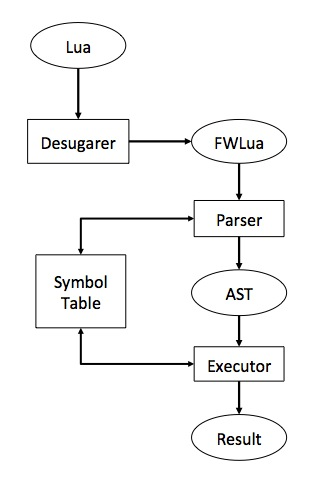
\includegraphics[scale = 0.9]{Interpreter}
\end{figure}

%\section{Desugaring in interpreter}
%Fortunately, there is a package named {\tt Text.ParserCombinators.Parsec} in Haskell, providing a set of functions for parsing tokens and thus building parsers. We will use this package to build the parser and ``desugarer''. Reference~\ref{instrucHAS} shows the details of this package.

%The key role in a functional programming language is recursive functions. Basically, this package allows us to parse token one by one recursively and thus control the data flow. According to this, our method to implement the desugaring is to parse every token in raw code, just like what parser does to code. What is different, this ``desugarer'' will transfer the inputs into another kind of code, instead of making an abstract syntax tree in parser. In other words, the file {\tt desugarer.hs} will take strings as token and then also return strings as new code. For example, we have discussed that the assignment statement in the global environment:

%\begin{verbatim}
%x = 42; --In Lua
%rawset("\_ENV", "x", 42); --equals to in FWLua
%\end{verbatim}
%And this is exactly the job of desugarer. Hence for, the code would be like following:
%\begin{verbatim}
%...
%assignmentStatement = do
%  ident <- identExpression
%  spaces
%  char '='
%  spaces
%  val <- expression
%  spaces
%  return $ "rawset(" ++ ident ++ ", " ++ val ++ ")"
%...
%\end{verbatim}
%
%We can see, it takes a set of tokens with the string type, and then returns a string as %``new code''.
%FIXME: paradigm again
%The paradigm of this block is based on the syntactic desugaring methods that we have mentioned previously. The FWLua code this block returns is used by the parser to create the AST.

\section{ParserTD.hs}
Fortunately, there is a package named {\tt Text.ParserCombinators.Parsec} in Haskell, providing a set of functions for parsing tokens and thus building parsers. We will use this package to build the parser. Reference~\ref{instrucHAS} shows the details of this package.

The key role in a functional programming language is recursive functions. Basically, this package allows us to parse token one by one recursively and thus control the data flow. According to this, the parser uses {\tt parsec} for passing tokens and it takes strings as tokens. Then it returns a tree --an abstract syntax tree (AST).
The AST is made up of different types of nodes.
%FIXED: Not sure I agree with the next sentence.  Let's discuss.
Technically, all nodes in the AST will exactly represent the whole program. Every time it parses a token, AST should be modified (even could be ``do nothing'').

%FIXME: This paragraph raises some read flags for me.  Let's discuss.
%FIXED: Deleted

The parser cares about the syntax of FWLua. In other words, there are no evaluations or storage manipulations in the parsing phase. The only purpose in this block is to sort the inputs by using the structure of the tree, and thus bring the cleaner AST to the executer. The AST is completely created by parser. It also means that we can handle different kinds of inputs by using different parsers with the same executor.

\section{Symbol Table}
Haskell is a strongly-typed programming language. Everything we want to define needs to have a type, and Haskell strickly follows this type. The tier of the symbol table stores all new types we define and it is used as a user-defined library.

%FIXED: Paradigm again
There are two ways declaring new data types in Haskell: {\tt data} and {\tt type}. The token {\tt type} allows us to define a new type with one single format, while the token {\tt data} defining a new variable type in multiple formats with different tokens. For instance, the part of code in the symbol table is shown:

%FIXED: Replace flushleft with verbatim wherever you are using it
\begin{verbatim}
type Store = Map Register Table
type Argument = String
data Value = 
    VNil
  | VArg String
  | VFunc Argument Expression
  | VResFunc String
  | VReg Register
  | VInt Integer
  | VBool Bool
  | VStr String
  | VTrue
  | VFalse
  deriving (Show)
\end{verbatim}

The type {\tt Store} and {\tt Argument} have the single typing paradigm. They don't need a specific token to be distinguished. On the contrary, the data {\tt Value} has multiple cases and thus needs different tokens (such as {\tt VArg}, {\tt VFunc} and {\tt VInt} in the code above).

\section{Executor.hs}
{\tt Executor.hs} represents the semantics of FWLua that we have given above. The function {\tt evaluate()} is the main function in the file. It takes different kinds of nodes in the AST for evaluating, then returns values and the manipulated store as the final result. There are also some other assisting reserved functions for helping the evaluation rules
%FIXED: We need to talk through this part
such as address allocation, key pointing, binary operation application and so on. At the beginning, the global store is supposed to be empty.

\section{Run and Runfile}
We have also built a run file to test if our interpreter works as intended. What is more, this file links all components that we introduced before. In the run file, we treat inputs as a string flow. Then it will parse it, execute the AST and finally output the results. The results include the desugared code, detail of the AST, the summary of store, and final results. Since it shows all the information that we need, we can debug our interpreter due to the outputs from this run file.
